%!TEX root =  ../main.tex

\indexedSection{Sets}\label{sec:Sets}

\objective{Manipulate and create sets and intervals using set-builder notation.}


In this section, we will review how to describe regions of numbers and sets.

\begin{derivation}{Set}
A \gls{set} is a well-defined collection of distinct objects, and is considered as an 
object in its own right.  ``Well-defined''
means it is readily apparent to anyone if an object is or is not part of the set.
\end{derivation}

An object in a set is called an ``element''.  If $A = \{1, 2, 5\}$ then the 
elements of $A$ are 1, 2, and 5\footnote{Notice that the convention is to
choose capital letters close to the start of the alphabet for set names, and then
delimit the entries in a comma-separated list, inside curly brackets.}.  We may
also say $5 \in A$, which pronounced aloud as ``five is an element 
of $A$''\footnote{You might remember this symbol
by noting how much it looks like a capital E, which is the first letter 
of ``element'', as in ``is an element of''.}.  If set $B$ is
defined as $B=\{1,2\}$, then we can say $B \subseteq A$, that is, ``$B$ is a 
subset of $A$''.  $\varnothing$ is the symbol for the 
null set, also called the empty set, i.e. the set with no elements.

With these tools for sets, we may define variables using \gls{set-builder notation}.  
For example, we might say:
\begin{equation}
\{ x | x > 0, x \in \{-3, -2, -1, 0, 1, 2, 3\}\}
\end{equation}


You should read A.1 if it were the prose paragraph, ``There is a variable $x$ such 
that $x$ is greater than 0, 
and $x$ is in the set from -3 to 3.''  Can you figure out what $x$ is actually equal to?  
All that was a very 
long way to write that $x = \{1,2,3\}$!  Why would anyone write this way?  
The power of this notation becomes
obvious later, when we bring in infinite sets.  To begin with, we will use ``. . .'' 
(called an ``ellipsis'') to make infinite sets that keep going as before.


\begin{derivation}{Set-Builder Notation}
A subject and a predicate, separated by a pipe and enclosed in curly-brackets.
\end{derivation}


\begin{example}
\exProblem
Use set-builder notation to describe all the odd numbers greater than 3.

\exSolution
Odd numbers are one unit away from even numbers, which are themselves two times \textit{any} number.
\begin{align*}
\{ x | x \in \{5, 7, 9, ...\} \} \\
\{ 2x + 1 | x \in \{2, 3, 4, ...\} \} \\
\{ 2x + 1 | x>2, x \in \{1, 2, 3, ...\} \} 
\end{align*}
\end{example}

\subsection{Union and Intersection}
Lastly, sets may be joined, looking only for the overlap, or united, look for anything in either.  
The overlap is called ``intersection'' and is symbolized with a $\cap$, while 
``anything in either'' is called ``union'' and
is symbolized with a $\cup$.  This can be most easily visualized via Venn diagrams:

\reminder{\lefthand}{$\cup$ is an easy symbol to memorize, since its name is
\textbf{u}nion, and it looks like a U.  You might consider intersection as it opposite.}



\begin{figure}[h]
\centering

    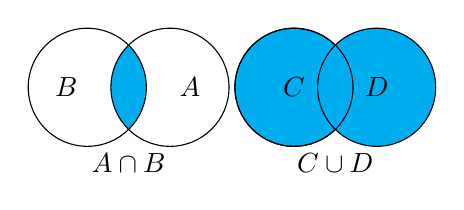
\begin{tikzpicture}[scale=0.3]
      \begin{scope}
    \clip (180:1.75cm) circle (2.5cm);
    \fill[cyan] (0:1.75cm) circle (2.5cm);
      \end{scope}
      \draw (0:1.75cm) circle (2.5cm) node[text=black,right] {$A$};
      \draw (180:1.75cm) circle (2.5cm) node [text=black,left] {$B$};
      \draw (0,-2.4) node [anchor=north] {$A \cap B$};

\draw[fill=cyan] (7,0) circle (2.5cm) node {$C$};
\draw[fill=cyan] (10.5,0) circle (2.5cm) node {$D$};
\draw (7,0) circle (2.5cm);
\draw (8.75,-2.4) node [anchor=north] {$C\cup D$};
    \end{tikzpicture}
\caption[Union]{Union and Intersection}
\end{figure}

\begin{example}
\exProblem
Given that that $A = \{1, 2, 3, 4, 5\}$, $B = \{-3, -1, 1, 3, 5\}$, and
$C = \{-1, 2, 3, 5, 6\}$, find $(A \cap C) \cup (B \cap C)$.

\exSolution
$A \cap C$ means ``What do $A$ and $C$ have in common?'', which is 1, 3, and 5.
$B \cap C$ means ``What do $B$ and $C$ have in common?", which is -1, 3, 5.
$\{1, 3, 5\} \cup \{-1, 3, 5\}$ means, ``What is in either one?", which is $\{-1, 1, 3, 5\}$.
\end{example}

\begin{figure}[h]
\centering
\def\firstcircle{(90:1.75cm) circle (2.5cm)}
  \def\secondcircle{(210:1.75cm) circle (2.5cm)}
  \def\thirdcircle{(330:1.75cm) circle (2.5cm)}
    \begin{tikzpicture}[scale=0.3]
      \begin{scope}
    \clip \secondcircle;
    \fill[cyan] \thirdcircle;
      \end{scope}
      \begin{scope}
    \clip \firstcircle;
    \fill[cyan] \thirdcircle;
      \end{scope}
      \draw \firstcircle node[text=black,above] {$A$};
      \draw \secondcircle node [text=black,below left] {$B$};
      \draw \thirdcircle node [text=black,below right] {$C$};
    \end{tikzpicture}
\caption[Venn]{$(A \cap C) \cup (B \cap C)$}
\end{figure}

\newpage

\ExSection{Exercises}
Use set builder notation, both mathematical and verbal.
\begin{exercises}{sec:Sets}
\prob[AASet1] Write each given set in the Set-Builder Form:
\subprob $\{2, 4, 6, 8, 10\}$
\subprob $\{2, 3, 5, 7, 11\}$
\subprob $\{$January, June, July$\}$
\subprob $\{$a, e, i, o, u$\}$
\subprob $\{$Tuesday, Thursday$\}$
\subprob $\{1, 4, 9, 16, 25\}$
\subprob $\{5, 10, 15, 20, 25, 30\}$



\prob[AASet2] Write the following sets in Set-Builder Form or Rule form:
\subprob $\{1, 3 5, 7, 9\}$
\subprob $\{16, 25, 36, 49, 64\}$
\subprob $\{$a, e, i, o, u$\}$
\subprob $\{$violet, indigo, blue, green, yellow, orange, red$\}$
\subprob $\{$January, March, May, July, August, October, December$\}$

 

\end{exercises}



